\documentclass{homeworg}
\usepackage{amsmath}
\usepackage{xcolor}

\title{Travail 8 - Circuits séquentiels}
\author{Wats Raphaël}

\begin{document}
\maketitle

\section{Le rappel de la fonction logique}
\begin{center}
    \huge
    $\overline{BC} + BC + A\overline{B}D$
\end{center}
\begin{center}
    \begin{tabular}{|l|c|r|r|r|}
        \hline
            A & B & C & D & Y\\
        \hline
            0 & 0 & 0 & 0 & 1\\
            0 & 0 & 0 & 1 & 1\\
            0 & 0 & 1 & 0 & 0\\
            0 & 0 & 1 & 1 & 0\\
            0 & 1 & 0 & 0 & 0\\
            0 & 1 & 0 & 1 & 0\\
            0 & 1 & 1 & 0 & 1\\
            0 & 1 & 1 & 1 & x\\
            1 & 0 & 0 & 0 & x\\
            1 & 0 & 0 & 1 & x\\
            1 & 0 & 1 & 0 & 0\\
            1 & 0 & 1 & 1 & 1\\
            1 & 1 & 0 & 0 & 0\\
            1 & 1 & 0 & 1 & 0\\
            1 & 1 & 1 & 0 & 1\\
            1 & 1 & 1 & 1 & x\\
        \hline
    \end{tabular}\\
    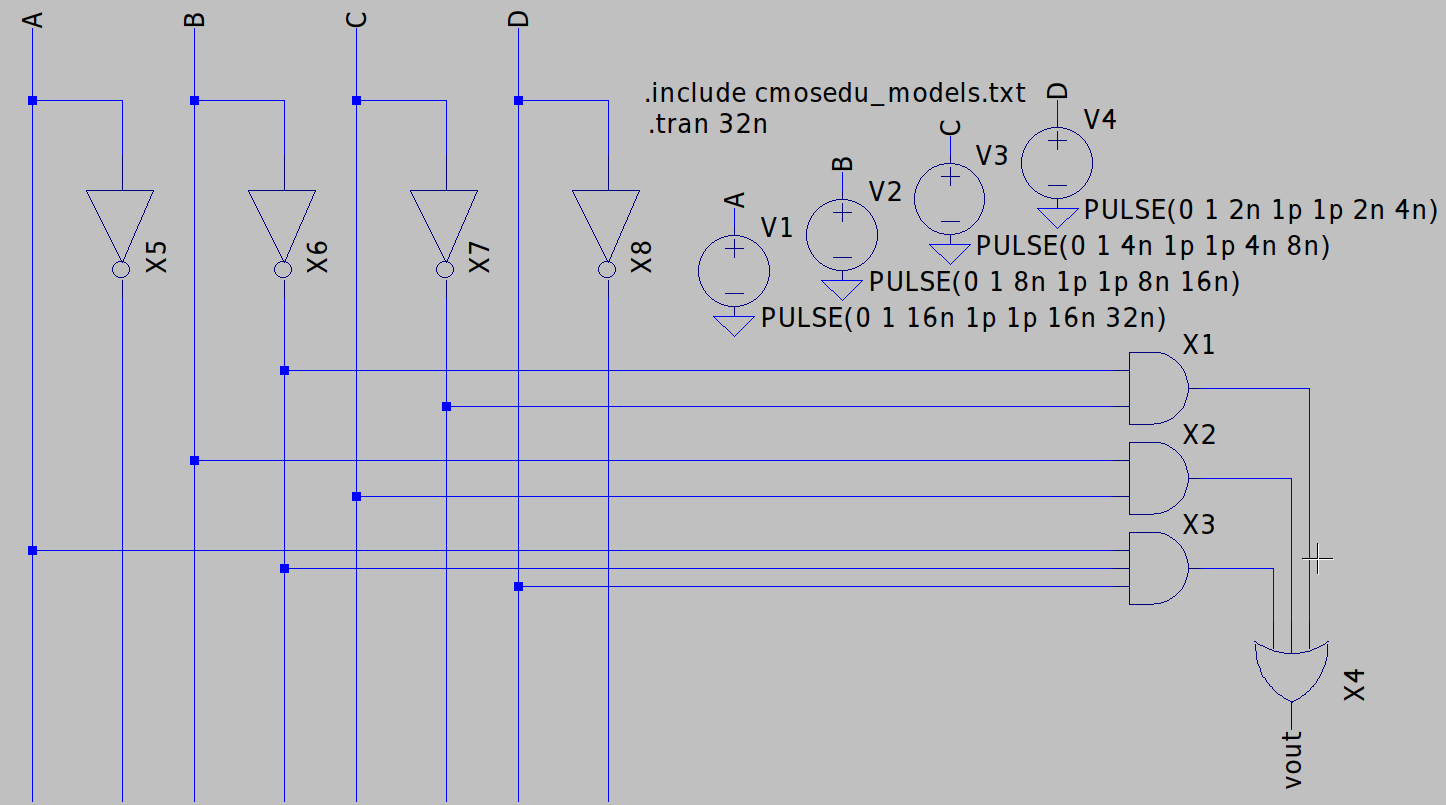
\includegraphics[scale=0.35]{circuit.png}
\end{center}
\newpage

\section{Le schéma du circuit}
\begin{center}
    \includegraphics[scale=0.5]{clocked.PNG}\\
\end{center}

\center Sous-circuit du DFF-4
\begin{center}
    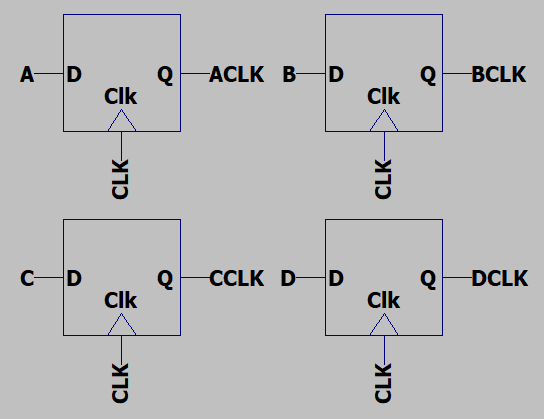
\includegraphics[scale=0.5]{dff4.PNG}\\
\end{center}

Implémentation CMOS de la fonction logique
\begin{center}
    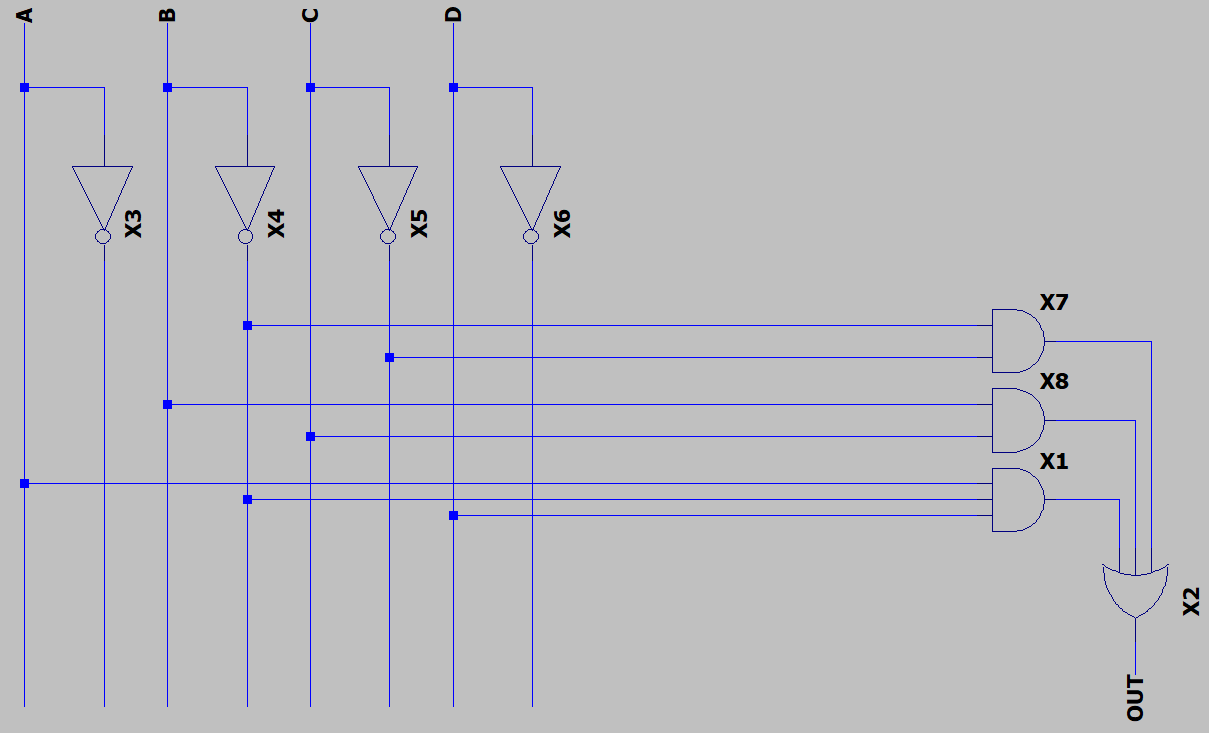
\includegraphics[scale=0.4]{fonction.PNG}
\end{center}
\newpage

\section{Le résultat de la simulation en parcourant la table de vérité}
\begin{center}
    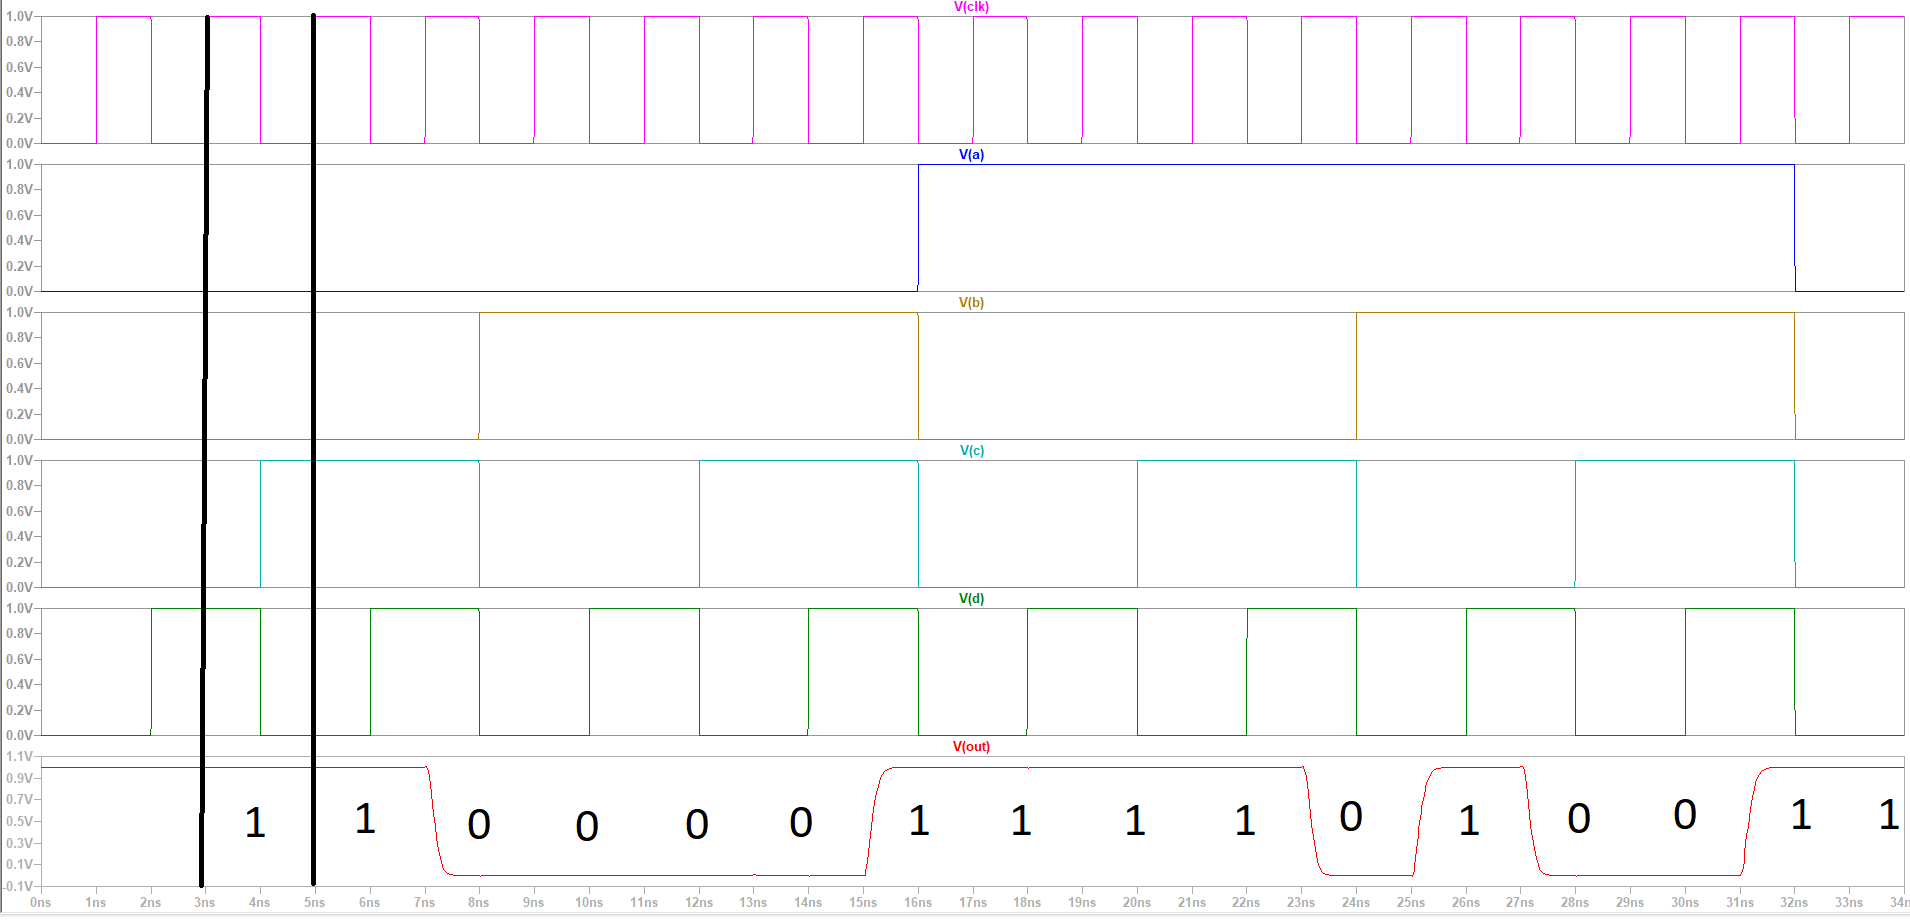
\includegraphics[scale=0.3]{truth.PNG}
\end{center}
L'utilisation de DFF dans un circuit séquentiel provoque un délai (ici de $2n$ secondes).

\section{Le résultat de la simulation à fréquence maximale}
Comme le temps de propgation du circuit est d'à peu près $0.4n$ secondes on obtient la fréquence maximum que l'horloge peut atteindre sans qu'il n'y ai de glitch à 2.5 GHz c'est à dire $1 / 0.4n = 2.5GHz$
\begin{center}
    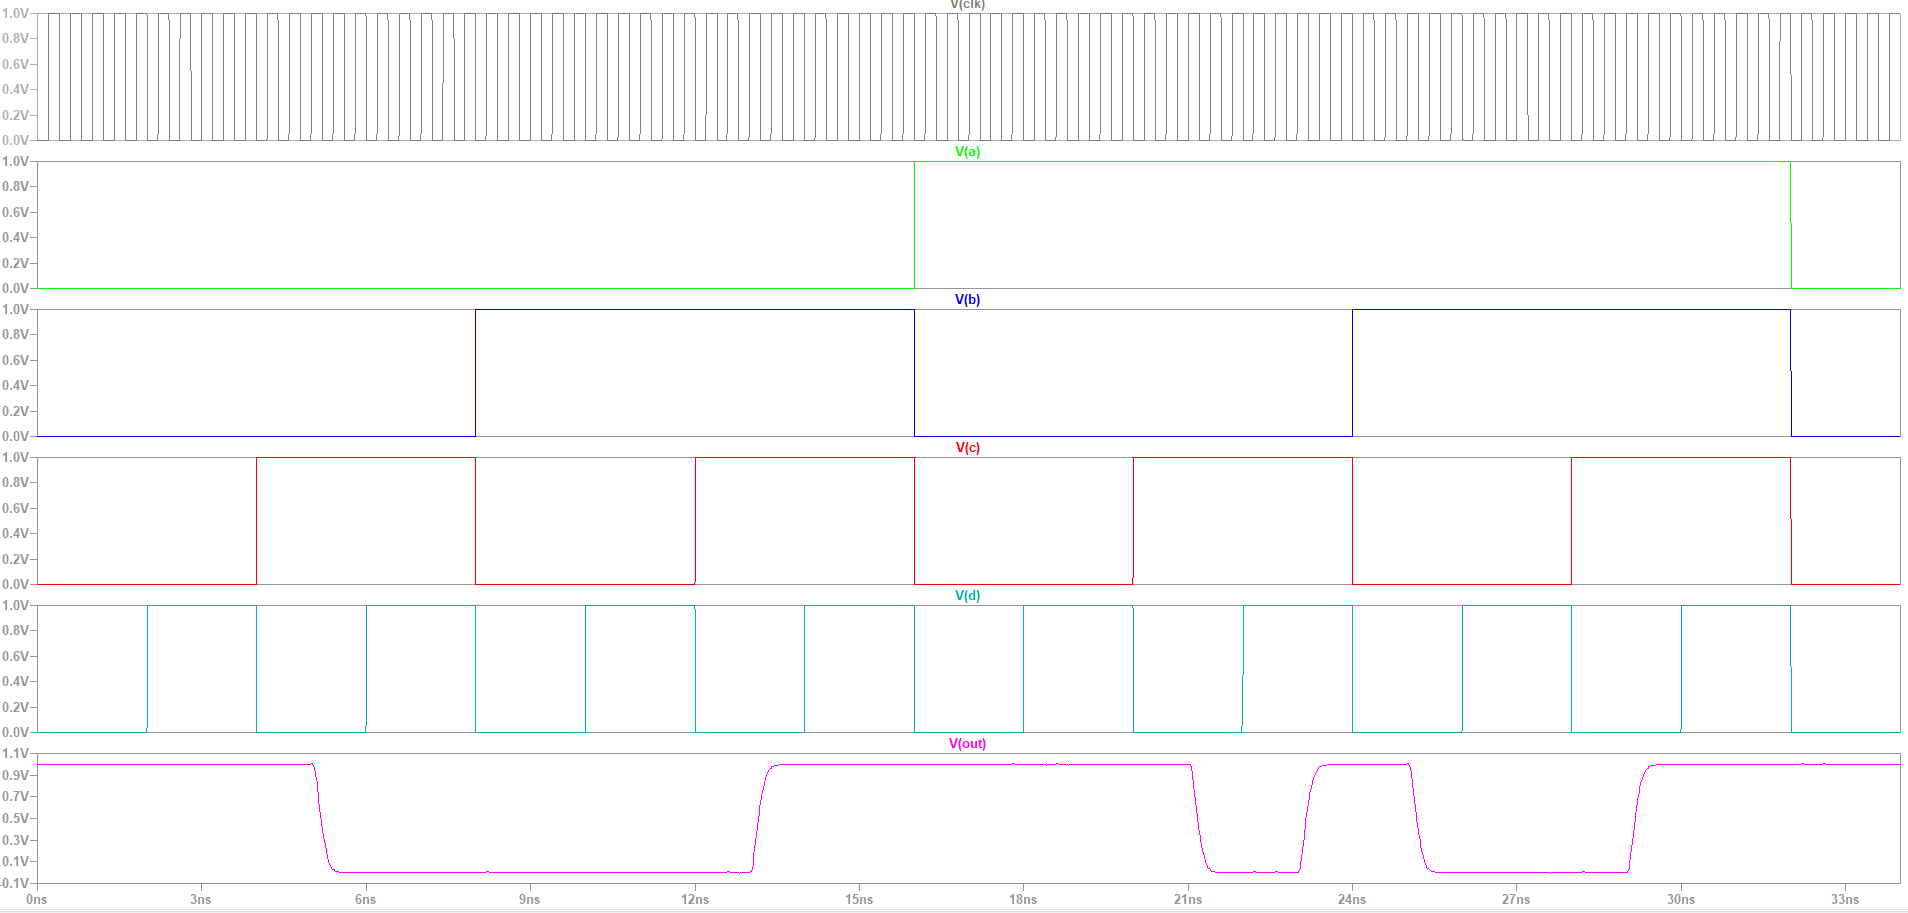
\includegraphics[scale=0.17]{truthMax.PNG}
\end{center}

Ci-dessous, on peut observer que lorsque le circuit est simulé avec une horloge réglée à une fréquence de 5GHz qui est une fréquence supérieur à la fréquence maximal de 2.5GHz, la tension de sortie commence à glitchée. On déduit donc que si l'on continue à augmenter la fréquence de l'horloge ces glitchs empêcherons d'apercevoir encore la table de vérité.
\begin{center}
    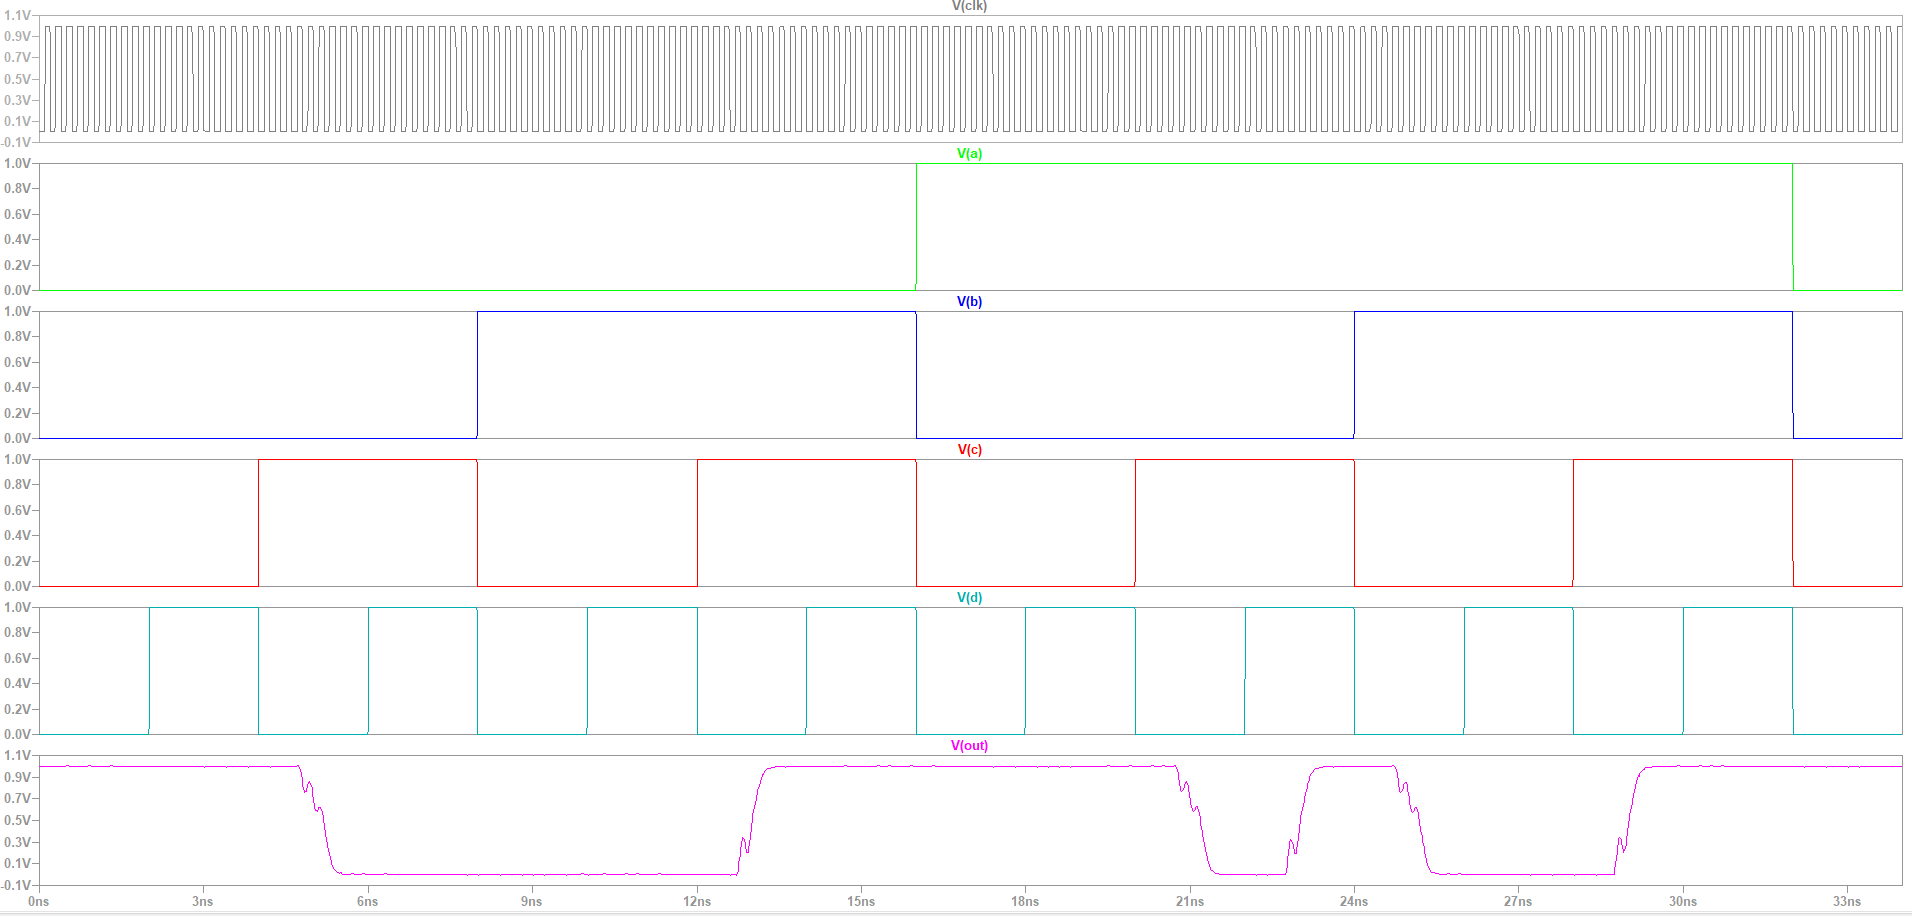
\includegraphics[scale=0.175]{truthExceed.PNG}
\end{center}
\newpage

\section{Conclusion}
Le temps de propagation estimé lors du travail précédent était d'à peu près $0.4n$ secondes, ce qui correspond à la période de la fréquence maximale à laquelle on peut régler l'horloge du circuit séquentiel proposé avant que la tension de sortie ne commence à glitcher d'où la relation suivante: $1/Tpd = Fmax$. Si l'on choisit une fréquence supérieur à la fréquence maximal supposée du circuit, le bruit généré pourrait causé des erreurs dans la logique d'un système complexe. Il est donc préférable de s'y tenir.
\end{document}
 
